\section{Result}
\label{sec:result}
We have tested our method on a corpus provided by teacher Xu. For detailed
description of the corpus, please see former report.

All the tests are conducted serval times (depending on computation cost,
vary from 5 to 20) with random selected training and testing speakers.
The average over these tests are considered as the final
result.

\subsection{Efficiency Test of our GMM}
We have extensively examined the efficiency of our implementation of GMM
compared to scikit-learn version. Test is conducted using real MFCC data with
13 dimensions. We consider the scenario when training a UBM with 256 mixtures.
We examine the time used for ten iteration.  For comparable results, we diabled
the K-means initialization process of both scikit-learn GMM implementation and
ours.  Time used for ten iterations under different data size and concurrency
is recorded.

\begin{figure}[!ht]
	\begin{minipage}{0.48\linewidth}
		\centering
		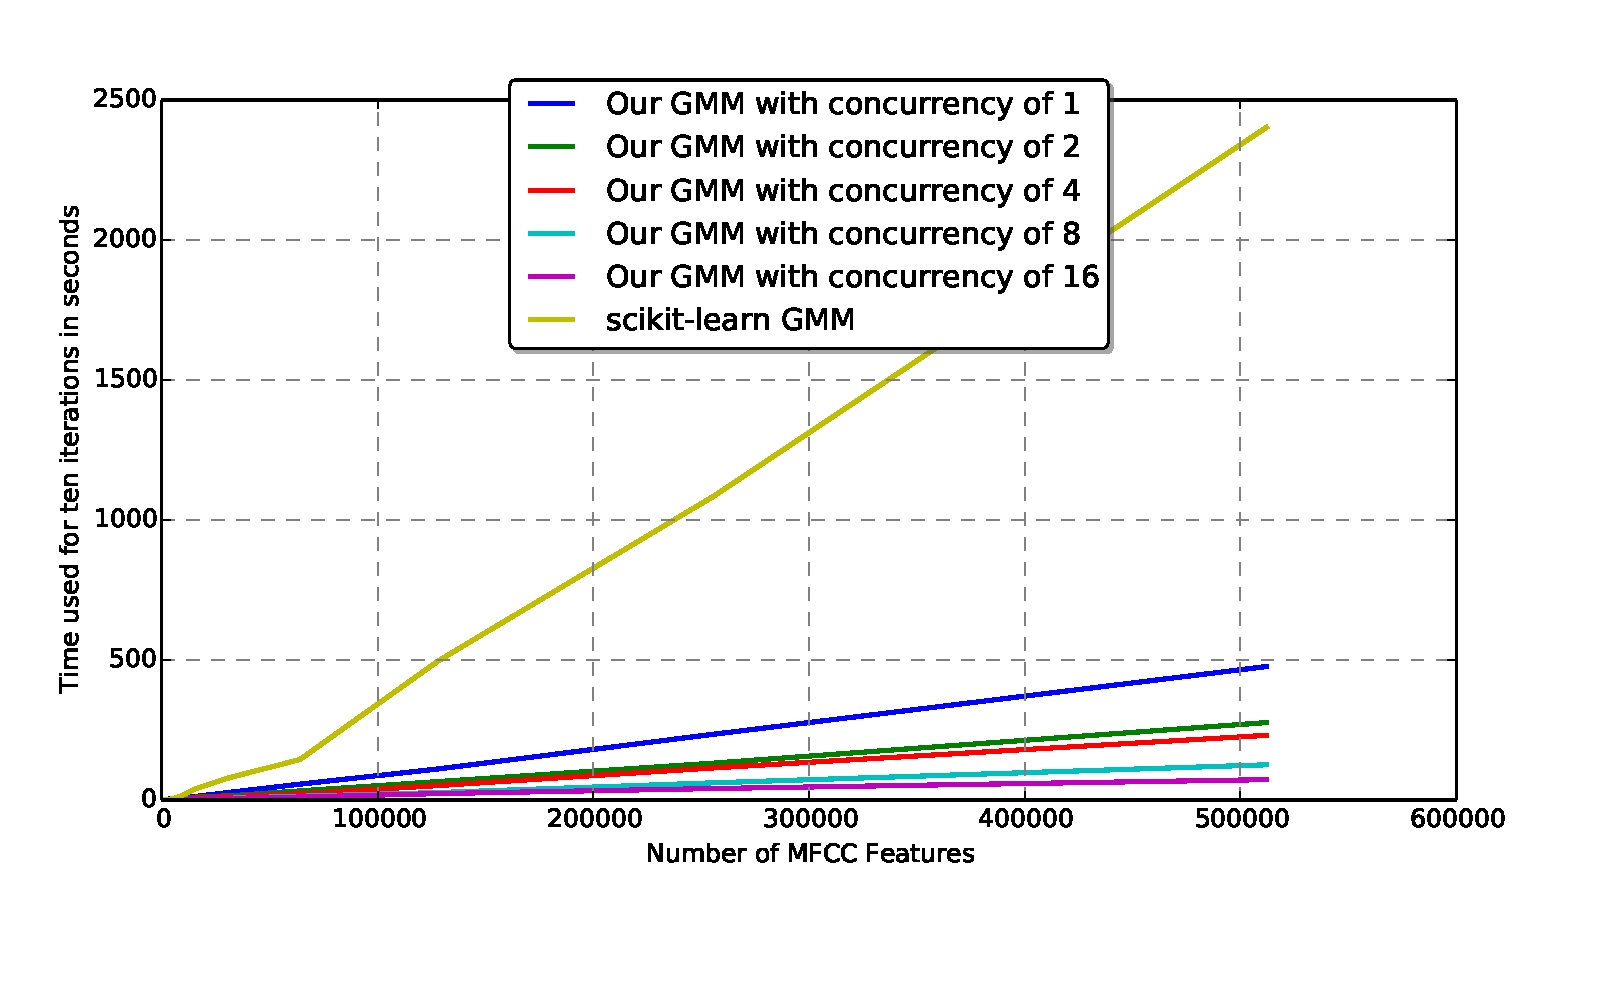
\includegraphics[width=\linewidth]{res/time-comp.pdf}
		\caption{Comparison on efficiency\label{fig:gmm_efficiency}}
	\end{minipage}
	\hfill
	\begin{minipage}{0.48\linewidth}
		\centering
		\includegraphics[width=\linewidth]{res/time-comp-small.pdf}
		\caption{Comparison on efficiency when number of MFCC features is small\label{fig:gmm_efficiency_small}}
	\end{minipage}
\end{figure}

From \figref{gmm_efficiency}, we can immediately infer that our method
is much-much more efficient than the widely used version of GMM provided
by scikit-learn when the data size grows sufficiently large.

We shall analyze in two aspect:
\begin{itemize}
	\item No concurrency
		\begin{itemize}
			\item When the number of MFCC features is below 6000, which is a typical
				number of features generated by 60 seconds utterances (1ms frame shift),
				our method is slightly slower; but this is trivial since
				1 minute utterance is too small.
			\item When the number of MFCC features grows sufficiently large, our method
				shows great improvement. When training 512,000 features, our method
				is 5 times faster than comparing method.
		\end{itemize}
	\item With concurrency \\
		Our method shows considerable concurrency scalability that the running time
		is approximately lineary to the number of cores using.

		When using 8-cores, our method is \textbf{$19$ times} faster than comparing
		method.
\end{itemize}


\subsection{Effect Of Number Of Mixtures}
We examined our GMM compared to GMM from scikit-learn.
Test is conducted on 30-speaker corpus, 30 seconds training utterance
and 100 random sampled 5 seconds test utterance for each speaker.

As \figref{mixture} illustrates, when number of mixtures is small,
our GMM outperforms scikit-learn version by $10\%$, which indicates our
GMM models the distribution more accurately. The maximum accuracy
happens when the number of mixtures is around 32, reaching $0.965$. As
the number of mixtures increases, the decrease in accuracy

\begin{figure}
	\centering
	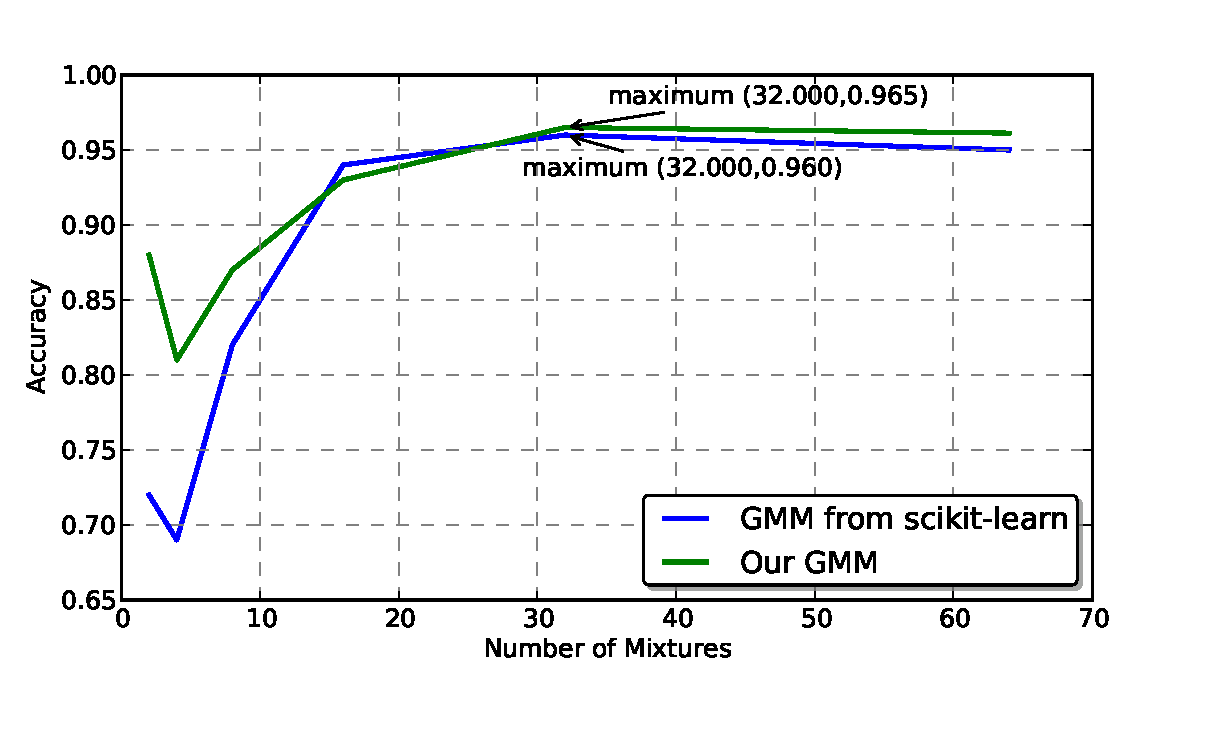
\includegraphics[width=\linewidth]{res/mixture-both.pdf}
	\caption{Accuracy curve on different number of mixtures\label{fig:mixture}}
\end{figure}

\section{Effect On Number Of Speakers}
An apparent trade-off in speaker recognition task is the number of speakers
enrolled and the accuracy of recognizing a person. We've conducted experiments
examining the effect of number of speakers enrolled on the performance of the
system.

The configurations of the test is as followed:
\begin{itemize}
	\item Number of mixtures is set to 32, the optimal number we found previously
	\item GMM from scikit-learn, compared to our GMM.
	\item 30s training utterance and 5s test utterance
	\item 100 sampled test utterance for each user
\end{itemize}


\begin{figure}[!ht]
	\centering
	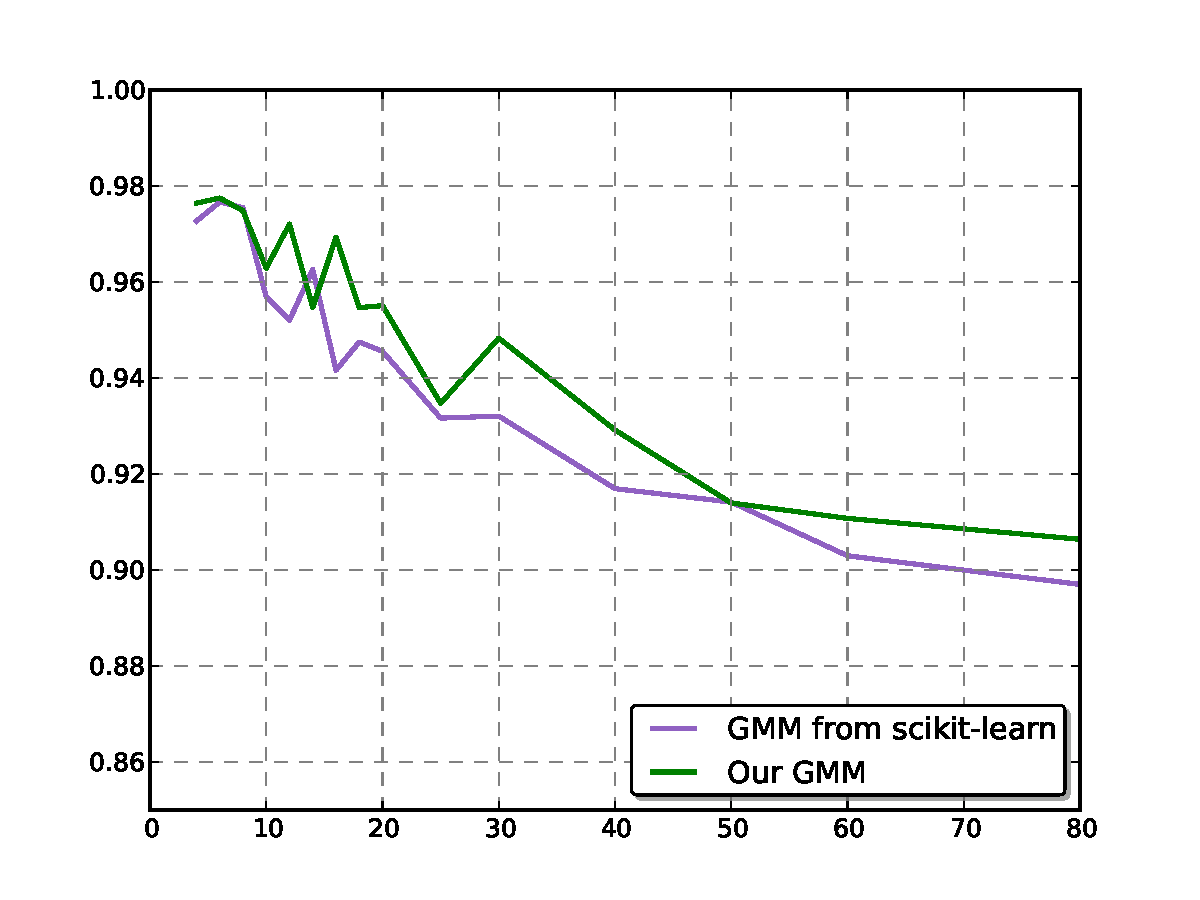
\includegraphics[width=\linewidth]{res/nperson.pdf}
	\caption{Accuracy curve on different number of speakers enrolled\label{fig:nspk_enrolled}}
\end{figure}

Scrunitizing \figref{nspk_enrolled} we would see that, our GMM performs better than
scikit GMM in general. When number of speakers is small, due to the the random
selection, the variance of the tests is significantly high, as we can see from the curve fluctuants.
When number of speakers increases, it is clear that the
accuracy of our GMM is above scikit version. As the more speaker, the more
difficult the recognition task will be, this result suggests that our
optimization on GMM takes effect.


